\chapter{SVG feature representation}\label{chap:features}
Our goal is to extend beyond polyline modeling and capture the higher-level shapes of SVG objects.
Thus, one major challenge is to choose an adequate representation that captures all drawing information from an SVG and can be fed as an input vector to our neural network architecture.
Although many different elements are allowed by the SVG specification, we simplify the problem space to focus only on \code{path}s (since \code{path}s can be used to compose other elements). 

\section{Overview of SVG commands}
There are five commands possible in an SVG \code{path} as seen in Figure~\ref{fig:svg-commands}. Further detail about command parameters can be found in Table~\ref{tbl:svg-commands}~\cite{grasso2011svg}.

\begin{figure}[h]
    \centering
	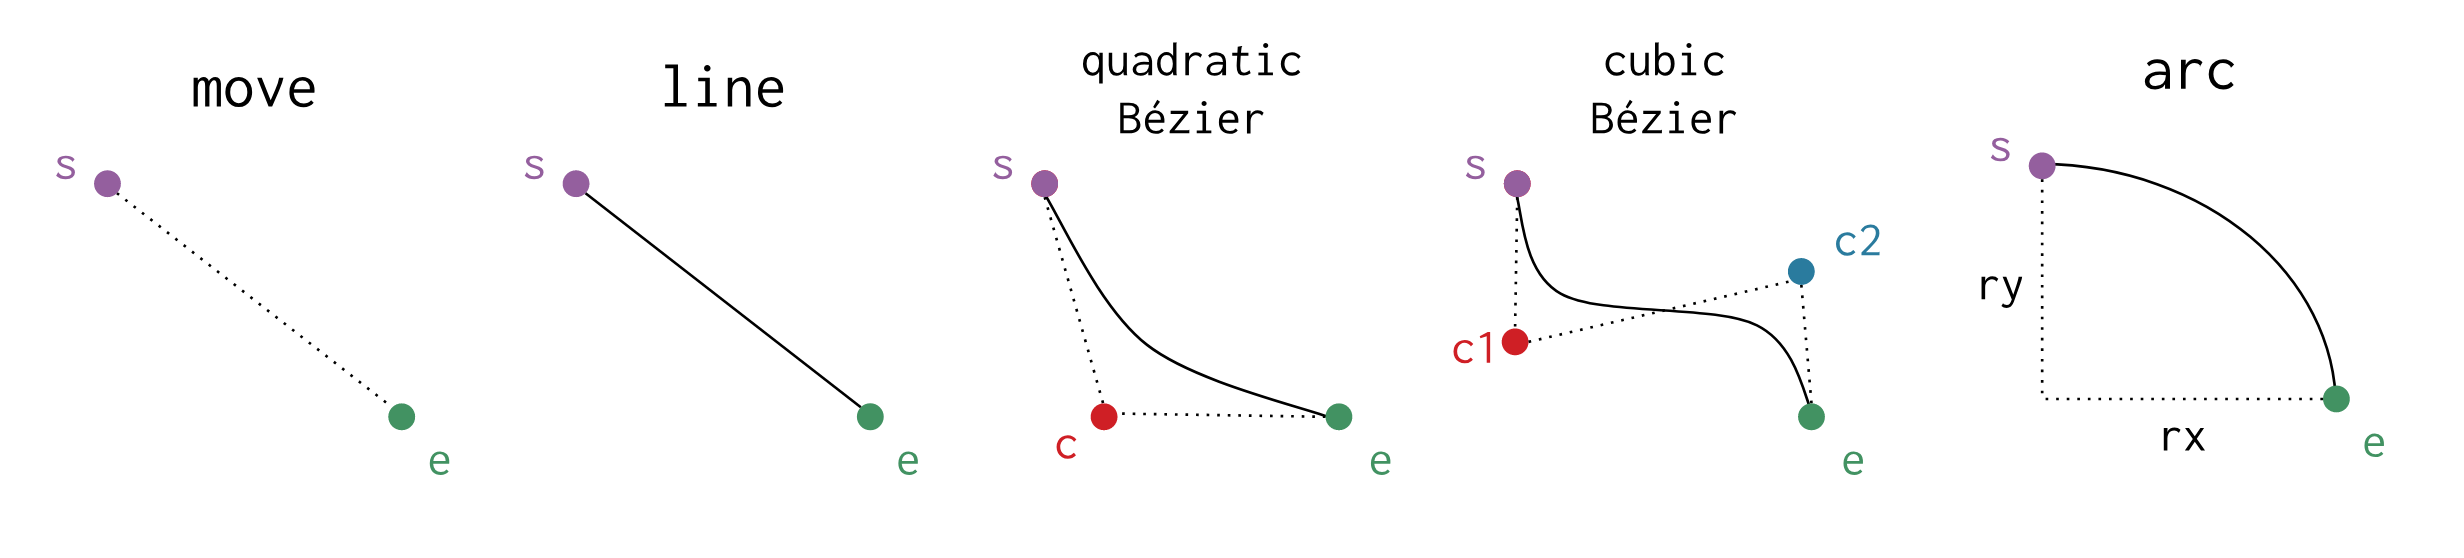
\includegraphics[width=\textwidth]{figures/commands}
    \caption{A visualization of the five commands in the SVG \code{path}\label{fig:svg-commands}}
\end{figure}


\begin{table}[h]
\centering
    \caption[The five possible commands in an SVG \code{path}]{A description of possible SVG path commands.
    For simplicity, we omit the relative coordinate variants of the commands, which specify relative $(dx, dy)$ coordinates instead of absolute $(x, y)$ for all pairs of control points.
    We also omit commands for vertical (\code{V}) and horizontal (\code{H}) lines as well as shorthand smoothed quadratic (\code{T}) and cubic (\code{S}) B\'eziers.\label{tbl:svg-commands}}
\begin{tabularx}{\linewidth}{l X}
\toprule
    Command & Description \& Code \\ \midrule
    Move & moves the pen to a specified point $(x, y)$ \\
    & \code{M x y} \\
    Line & draws a line from the current (start) point to the end point $(x, y)$ \\
    & \code{L x y} \\
    Quadratic B\'ezier & draws a quadratic curve according to given control point $(cx, cy)$ from the current point to the end point $(x, y)$ \\
    & \code{Q cx cy, x y} \\
    Cubic B\'ezier & draws a cubic curve according to given control points $(cx_1, cy_1)$ and $(cx_2, cy_2)$ from the current point to the end point $(x, y)$ \\
    & \code{C cx1 cy1, cx2 cy2, x y} \\
    Arc & draws a section of an ellipse with the given $r_x$ and $r_y$ radii from the current point to the end point $(x, y)$ over angle $t$, with large-arc $f_l$ and sweep $f_s$ flags \\
    & \code{A rx ry t fl fs x y}
\end{tabularx}
\end{table}


\section{Modeling SVGs}
We would like to model SVG inputs without loss of information about pen movements.
In essence, since SVGs name ordered lists of paths and their drawing commands, we model them as a sequence of mathematical parameters for the pen drawing commands and add a command for representing the transition between paths.
The sequential nature of this representation makes the generation task well-suited to a recurrent neural network architecture, as we cover in Section~\ref{sec:architecture}.

\subsection{Preprocessing}
SVG icons and font glyphs often have additional properties like stroke and fill style.
As we focus on path generation exclusively, our first step in transforming input SVGs is to strip away those styles and focus only on the \code{path} elements of the input, often resulting in an image that depicts the outlines of the input shape---see Figure~\ref{fig:input_fonts} for examples.

Often, designers do not craft SVGs by editing XML by hand but rather with interactive image editing software such as Adobe Illustrator or Inkscape (\TODO{citations?}).
Thus, human-created SVGs often have varying path compositions, viewboxes, and canvas sizes.

To constrain the generation process slightly, we first homogenize our dataset by preprocessing inputs to rescale to the same overall canvas size (set to $256\times 256$ pixels) as well as reorder paths in the drawing sequence so that paths with larger bounding boxes are drawn first.

There is also variability in the direction of path drawing and in starting positions. Instead of controlling these factors in the preprocessing stage, our architecture is designed for bidirectionality, and all command sequences are prepended such that the pen starts at coordinate $(0, 0)$.

\subsection{Simplifying path commands}
We aim to produce a system capable of modeling general SVGs, so inputs can contain all path commands specified in Table~\ref{tbl:svg-commands}.
To avoid bias and to constrain the problem space (\TODO{wording?}), we consolidate the different path commands into a single feature representation.
\TODO{this justification makes more sense with the dataset statistics of icons, but fonts use only quadratic beziers--how to better justify why we convert arcs to cubic beziers even though that's not a lossless process?}

Out of the five SVG path commands, three are parametic equations of differing degrees, so we can model these three (lines, quadratic B\'eziers, and cubic B\'eziers) using the parameter space for the highest degree cubic-order equation.
An elliptical arc segment, on the other hand, cannot be perfectly transformed into a cubic B\'ezier. Arcs have five extra parameters used to describe them ($x$-radius, $y$-radius, angle of rotation, the large arc flag, and the sweep flag), but they occur relatively rarely in the dataset, so it makes sense to approximate them with the same parameter space as used for our parametric commands.
We use the following method to approximate arc segments as cubic B\'eziers:

\begin{enumerate}
    \item Extract the arc parameters: start coordinates, end coordinates, ellipse major and minor radii, rotation angle from $x$ and $y$ axes, large arc flag, and sweep flag. 
    \item Transform ellipse into unit circle by rotating, scaling, and translating, and save those transformation factors.
    \item Find the arc angle from the transformed start point to end point on the unit circle.
    \item If needed, split the arc into segments, each covering an angle less than $90^\circ$.
    \item Approximate each segment angle's arc on a unit circle such that the distance from the circle center to the arc along the angle bisector of the arc is equal to the radius, defining cubic B\'ezier control points.
	\item Invert the transformation above to convert arcs along the unit circle back to the elliptical arc, transforming the generated control points accordingly.
	\item Use these transformed control points to parameterize the output cubic B\'ezier curve.
\end{enumerate}

After all path drawing command types have been transformed to use the parameters needed for modeling cubic B\'ezier segments, we can represent each SVG command as a feature vector comprising those parameters and a three-dimensional one-hot pen state vector, similar to the feature representation used in~\cite{ha2017neural}.

Finally, for each \code{move} command and each disjoint path, we insert a feature vector that encodes the new end point and sets the pen state to note that the pen is up.

In all, our feature representation models each drawing command as a nine-dimensional vector (in contrast to the five-dimensional feature vector for polyline drawings in~\cite{ha2017neural}).
Six dimensions are used to model three $x, y$ coordinate parameters of cubic B\'eziers, and three dimensions are reserved for the pen up ($p_u$), pen down ($p_d$), and end drawing ($p_e$) pen states.
Each input SVG is transformed into a sequence of commands, which is in turn translated into a sequence of these feature vectors.
In Chapter~\ref{chap:feature-variation}, we examine the details of this feature transformation process and how its tweaks affect modeling performance.
